\section*{Step 3}

\begin{custombox}[label={box:Q3}]{Step 3}
	Generate outputs by setting \textbf{degree = 1}, \textbf{degree = 3}, \textbf{degree = 6}, \textbf{degree = 10}, in the \verb|PolynomialFeatures| function used in \verb|E3.ipynb| and analyze them as follows:
	\begin{enumerate}[label=(\alph*)]
		\item Review the \verb|augmented_data.csv| file generated in each case and document your observations.
		\item Create an overall qualitative summary based on a review and analysis of the Figures generated.
		\item Summarize and explain the variations in the metrics \textbf{across regression methods for a given degree} (ie. a given set of polynomial features). Cover both, train and test, metrics, and compare them.
		\item Summarize and explain the variations in the metrics \textbf{across degrees for a given regression method}. Cover both, train, and test metrics, and compare them.
		\item When \textbf{degree = 1} which method(s) result in acceptable regression models? Why?
		\item When \textbf{degree = 6} which method(s) result in acceptable regression models? Why?
		\item As the value of degree is increased to 10 which regression methods show the most impact? Why?
		\item Why do non-parametric methods like \verb|KNN| and \verb|Decision Tree| based methods generate good results even without feature engineering?
		\item What are the limitations of the non-parametric methods?
		\item  Given the results, should LinearRegression be used at all? Why, when? Justify your answer.
	\end{enumerate}
\end{custombox}

\begin{figure}[H]
	\centering
	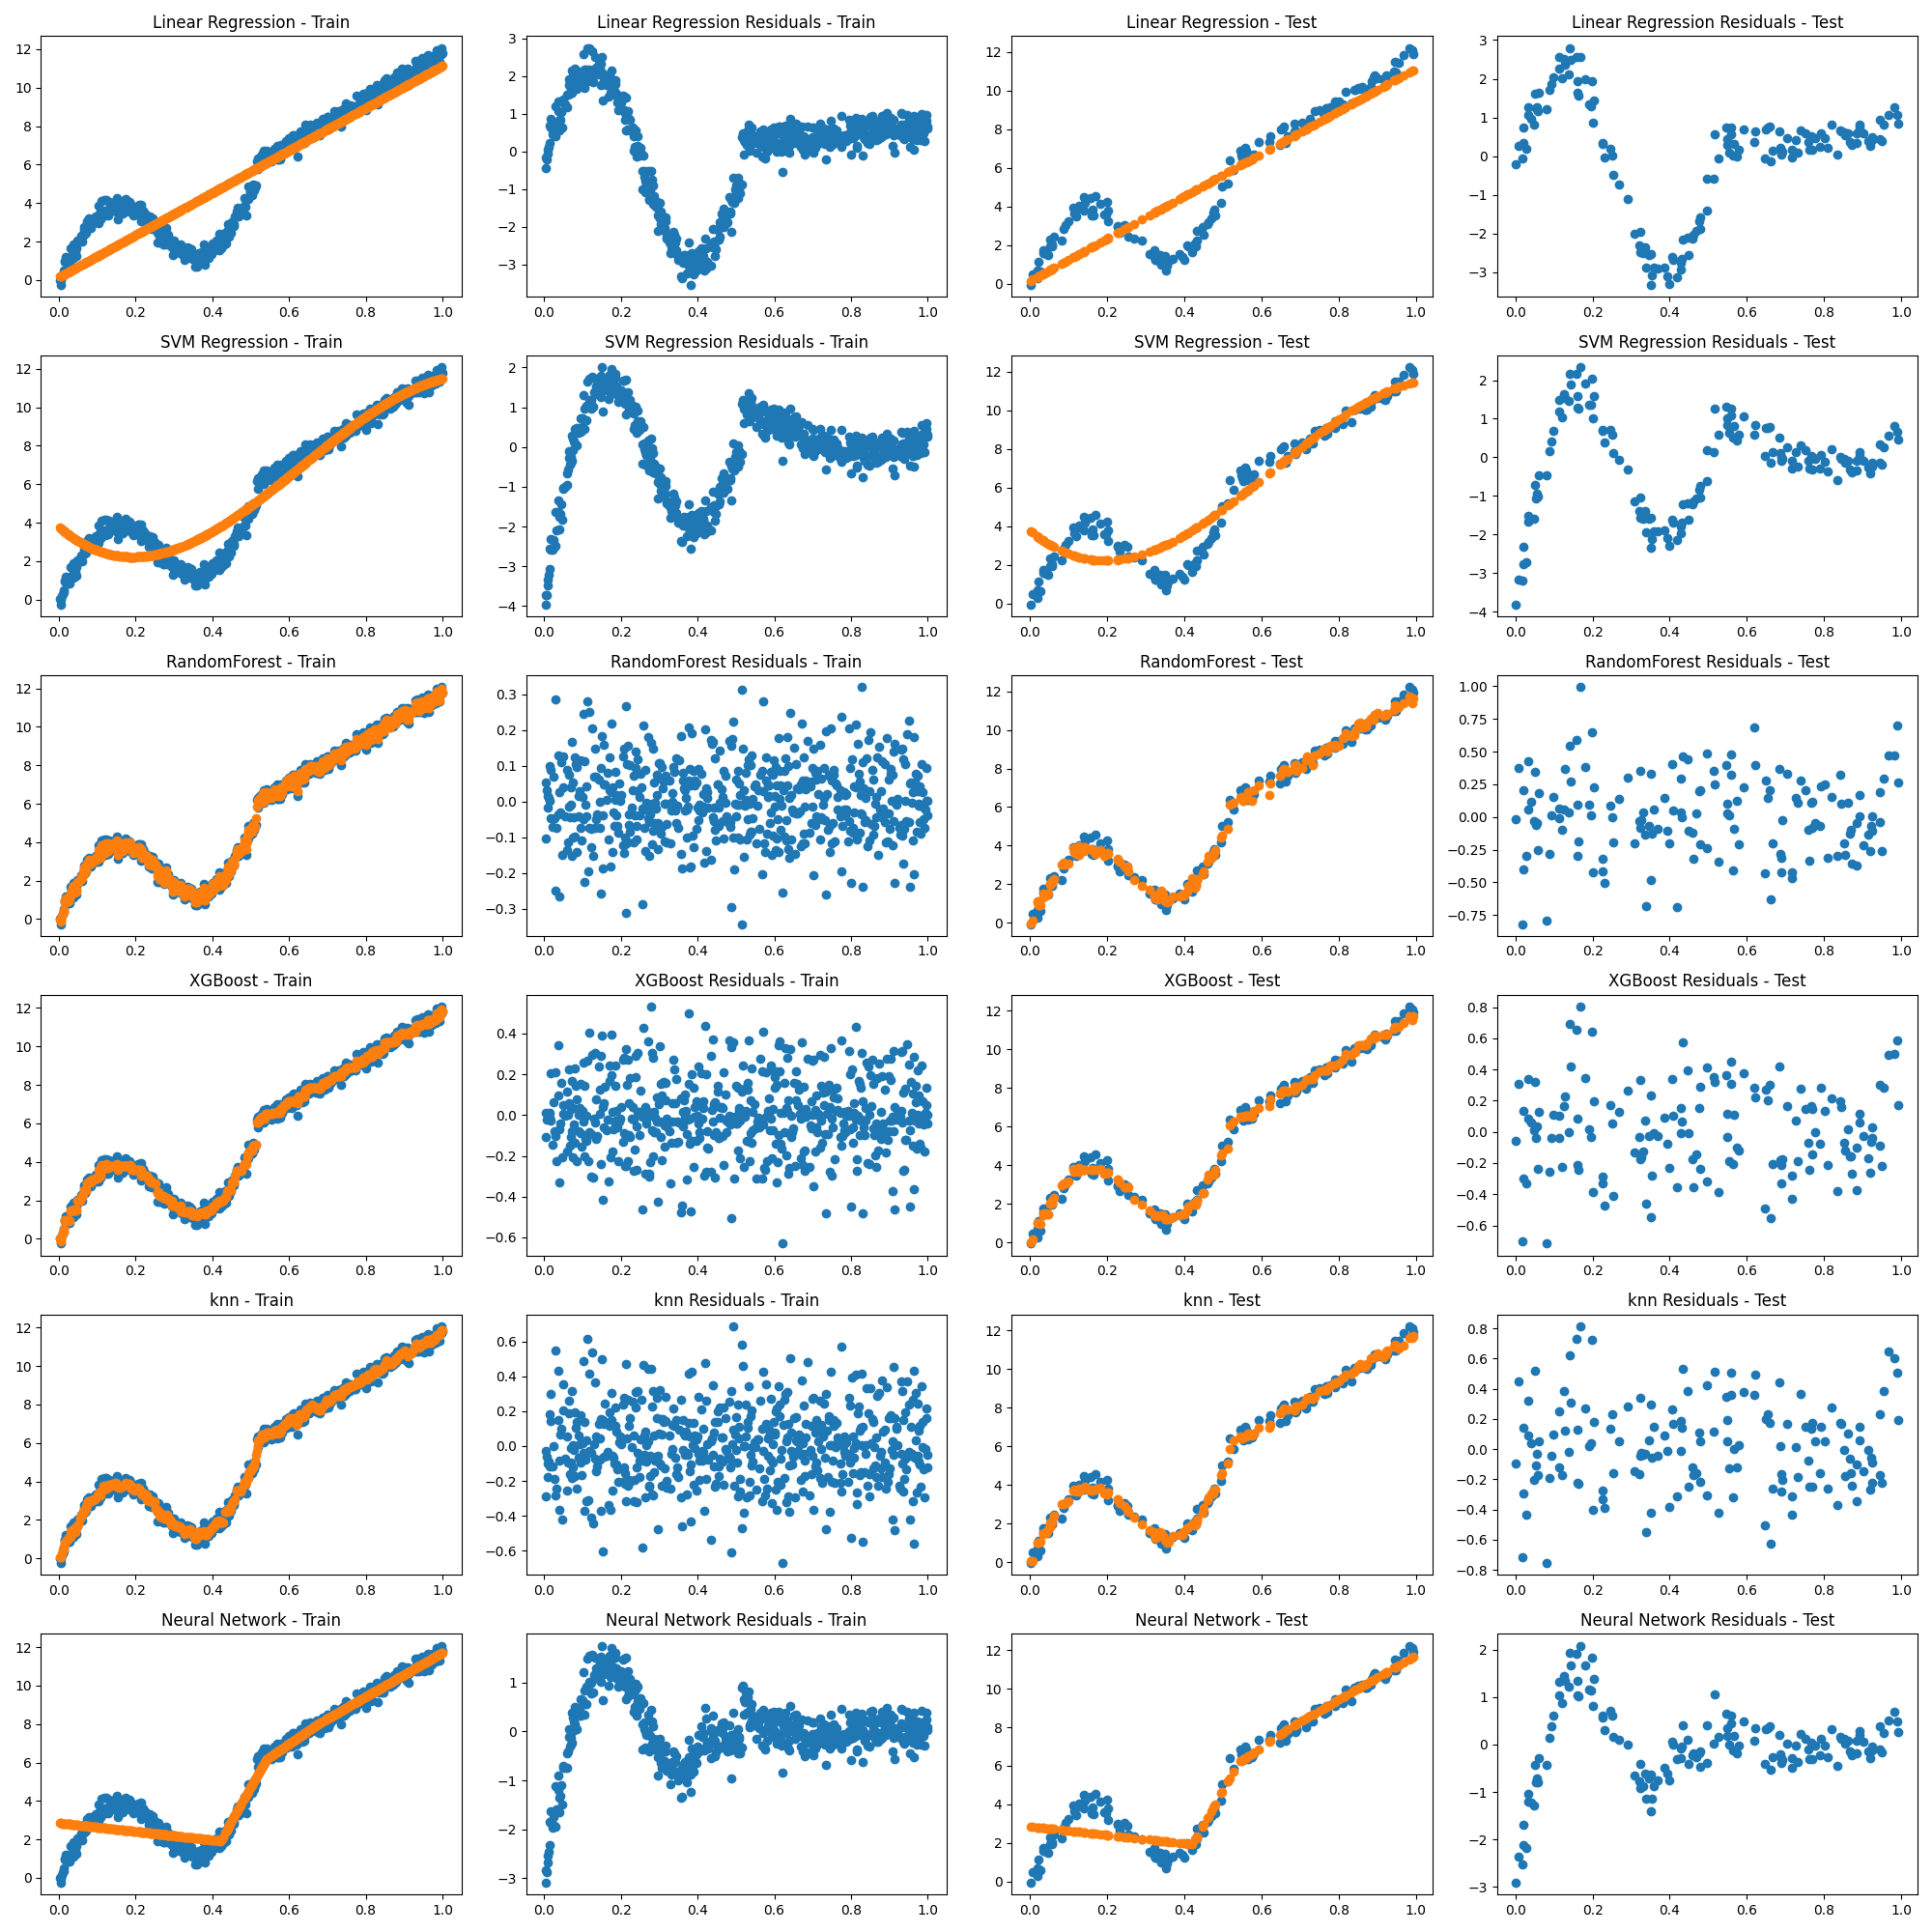
\includegraphics[width=\linewidth]{./Images/E3-MLR3-1.png}
	\caption{Various Regression Models with degree = 1}
\end{figure}

When degree = $1$, the following observations can be made:

\begin{itemize}
	\item The Linear Regression model is the best fit for the data.
	\item The Support Vector Machine (SVM) Regression model is the second-best fit for the data.
	\item The Random Forest, Gradient Boosting, K-Nearest Neighbors (KNN), and Neural Networks models are not good fits for the data.

\begin{figure}[H]
	\centering
	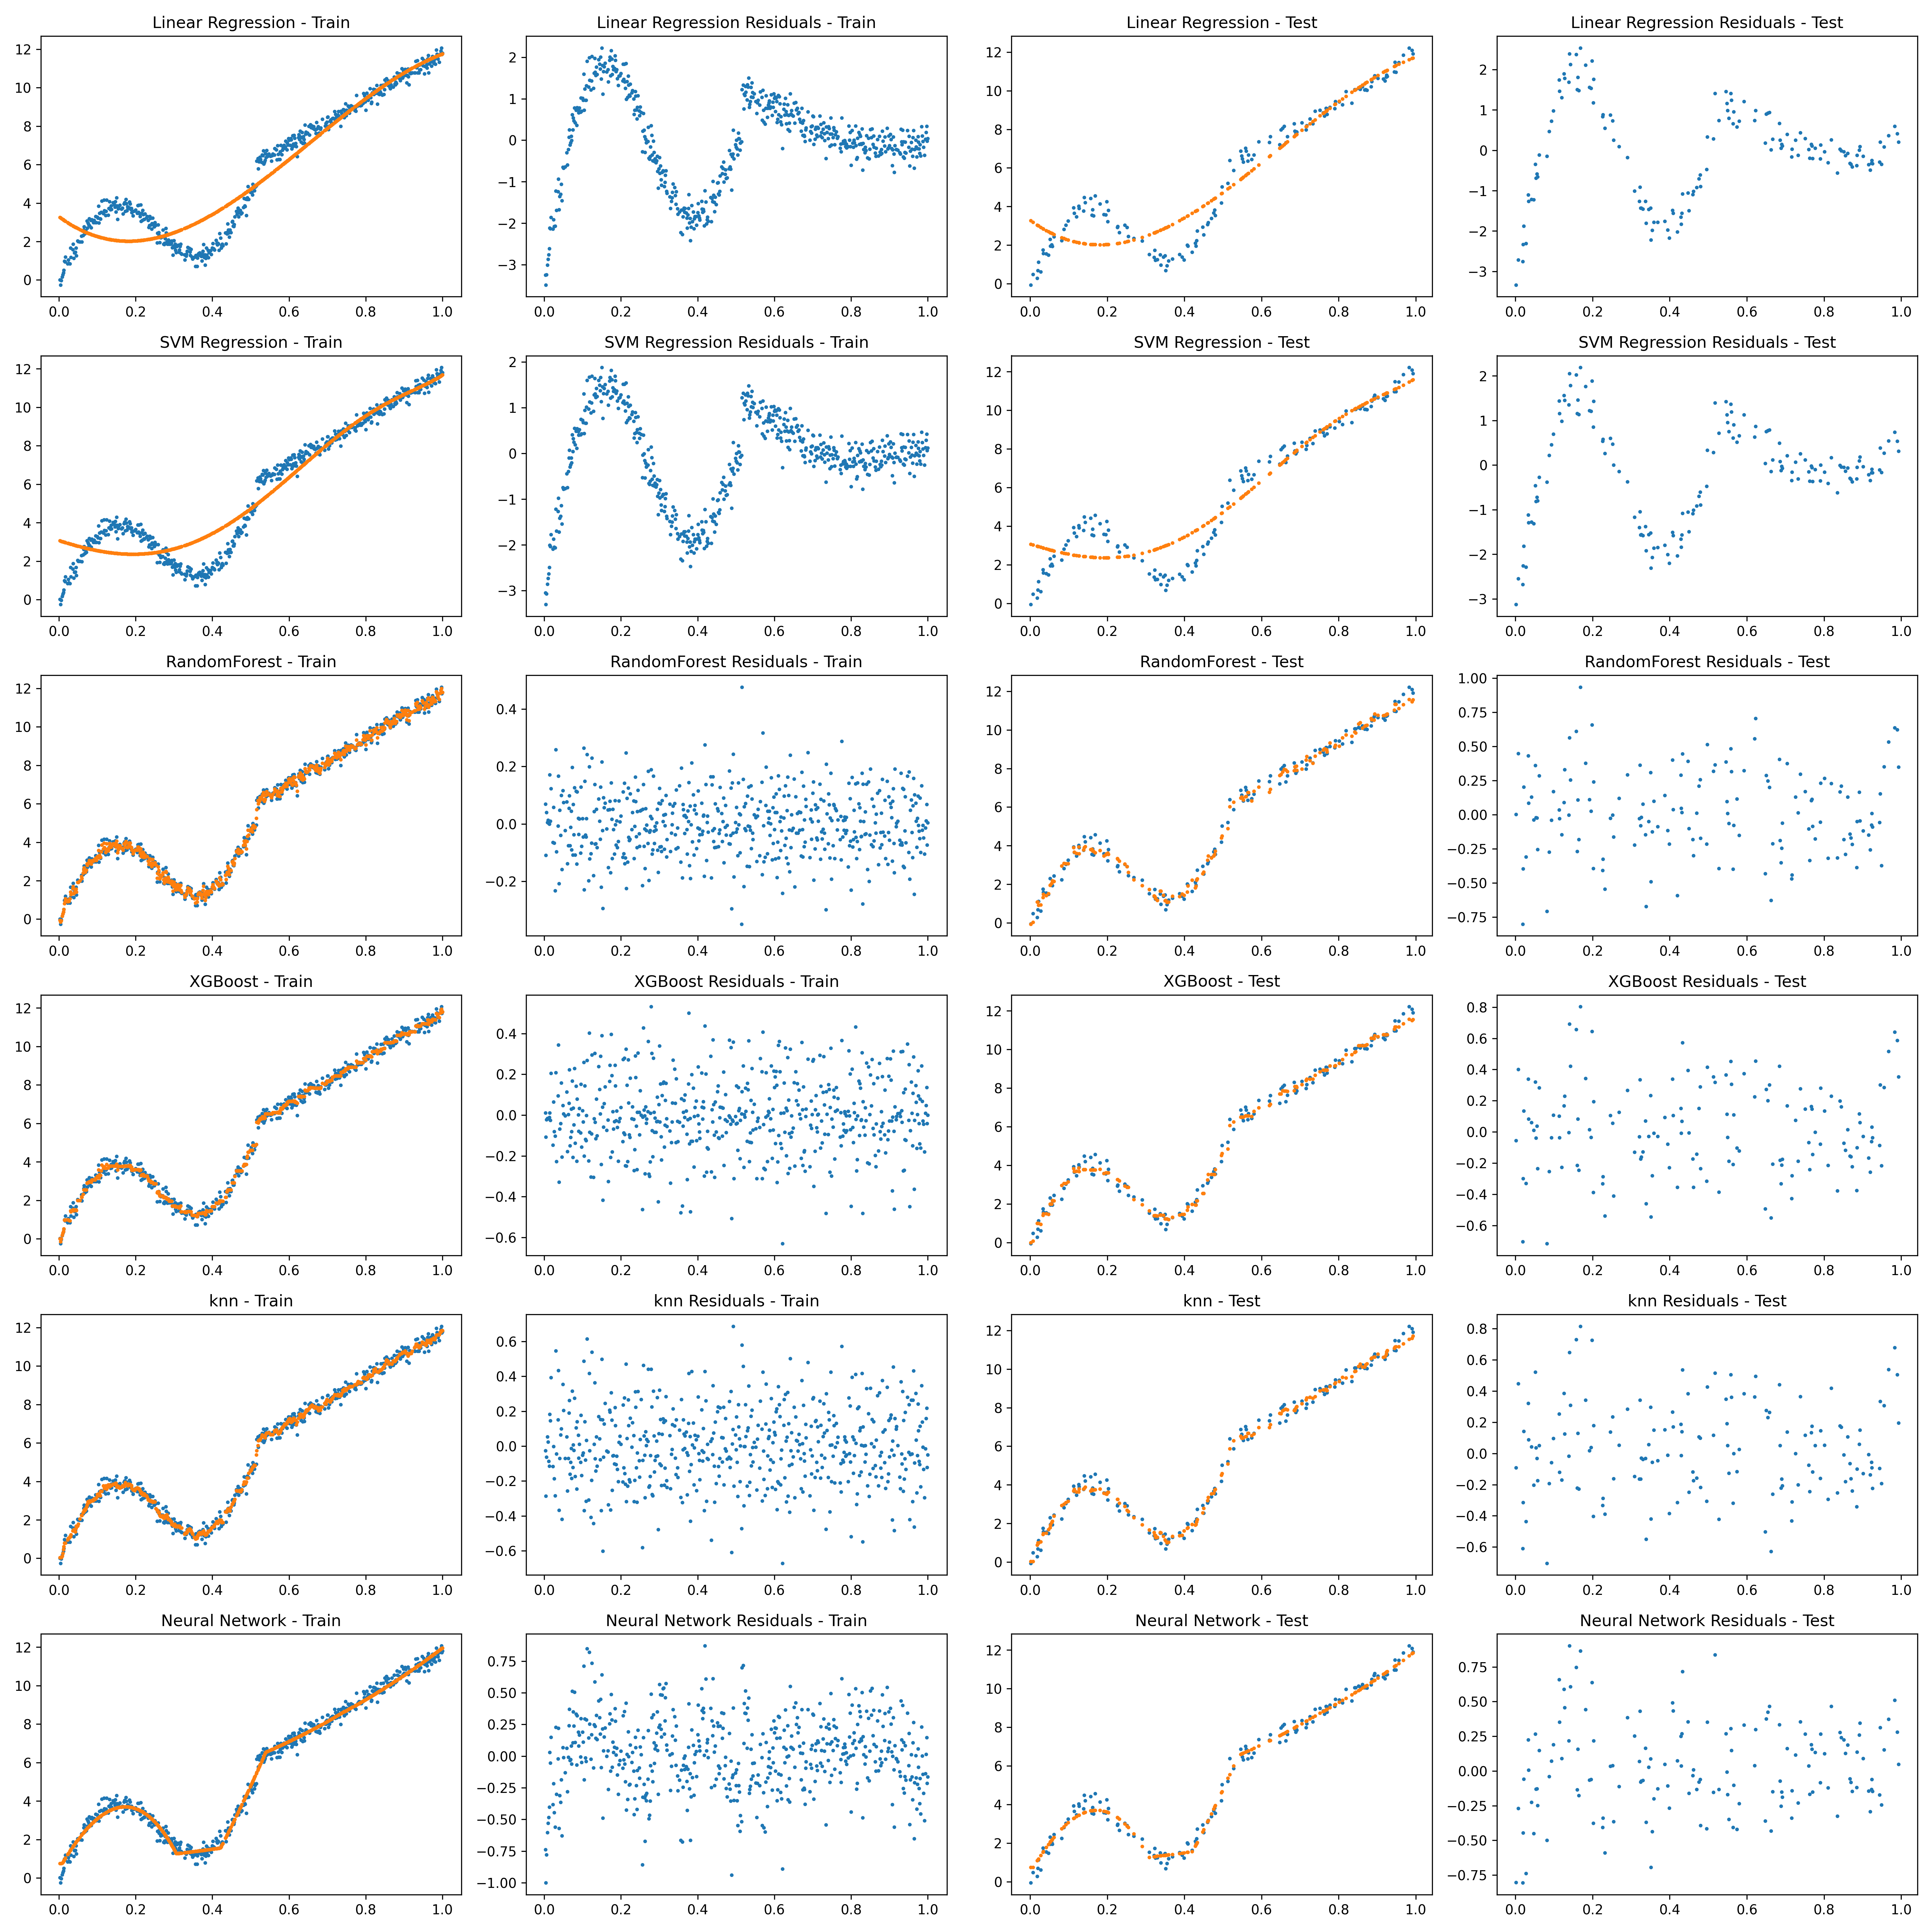
\includegraphics[width=\linewidth]{./Images/E3-MLR3-3.png}
	\caption{Various Regression Models with degree = 3}
\end{figure}

\begin{figure}[H]
	\centering
	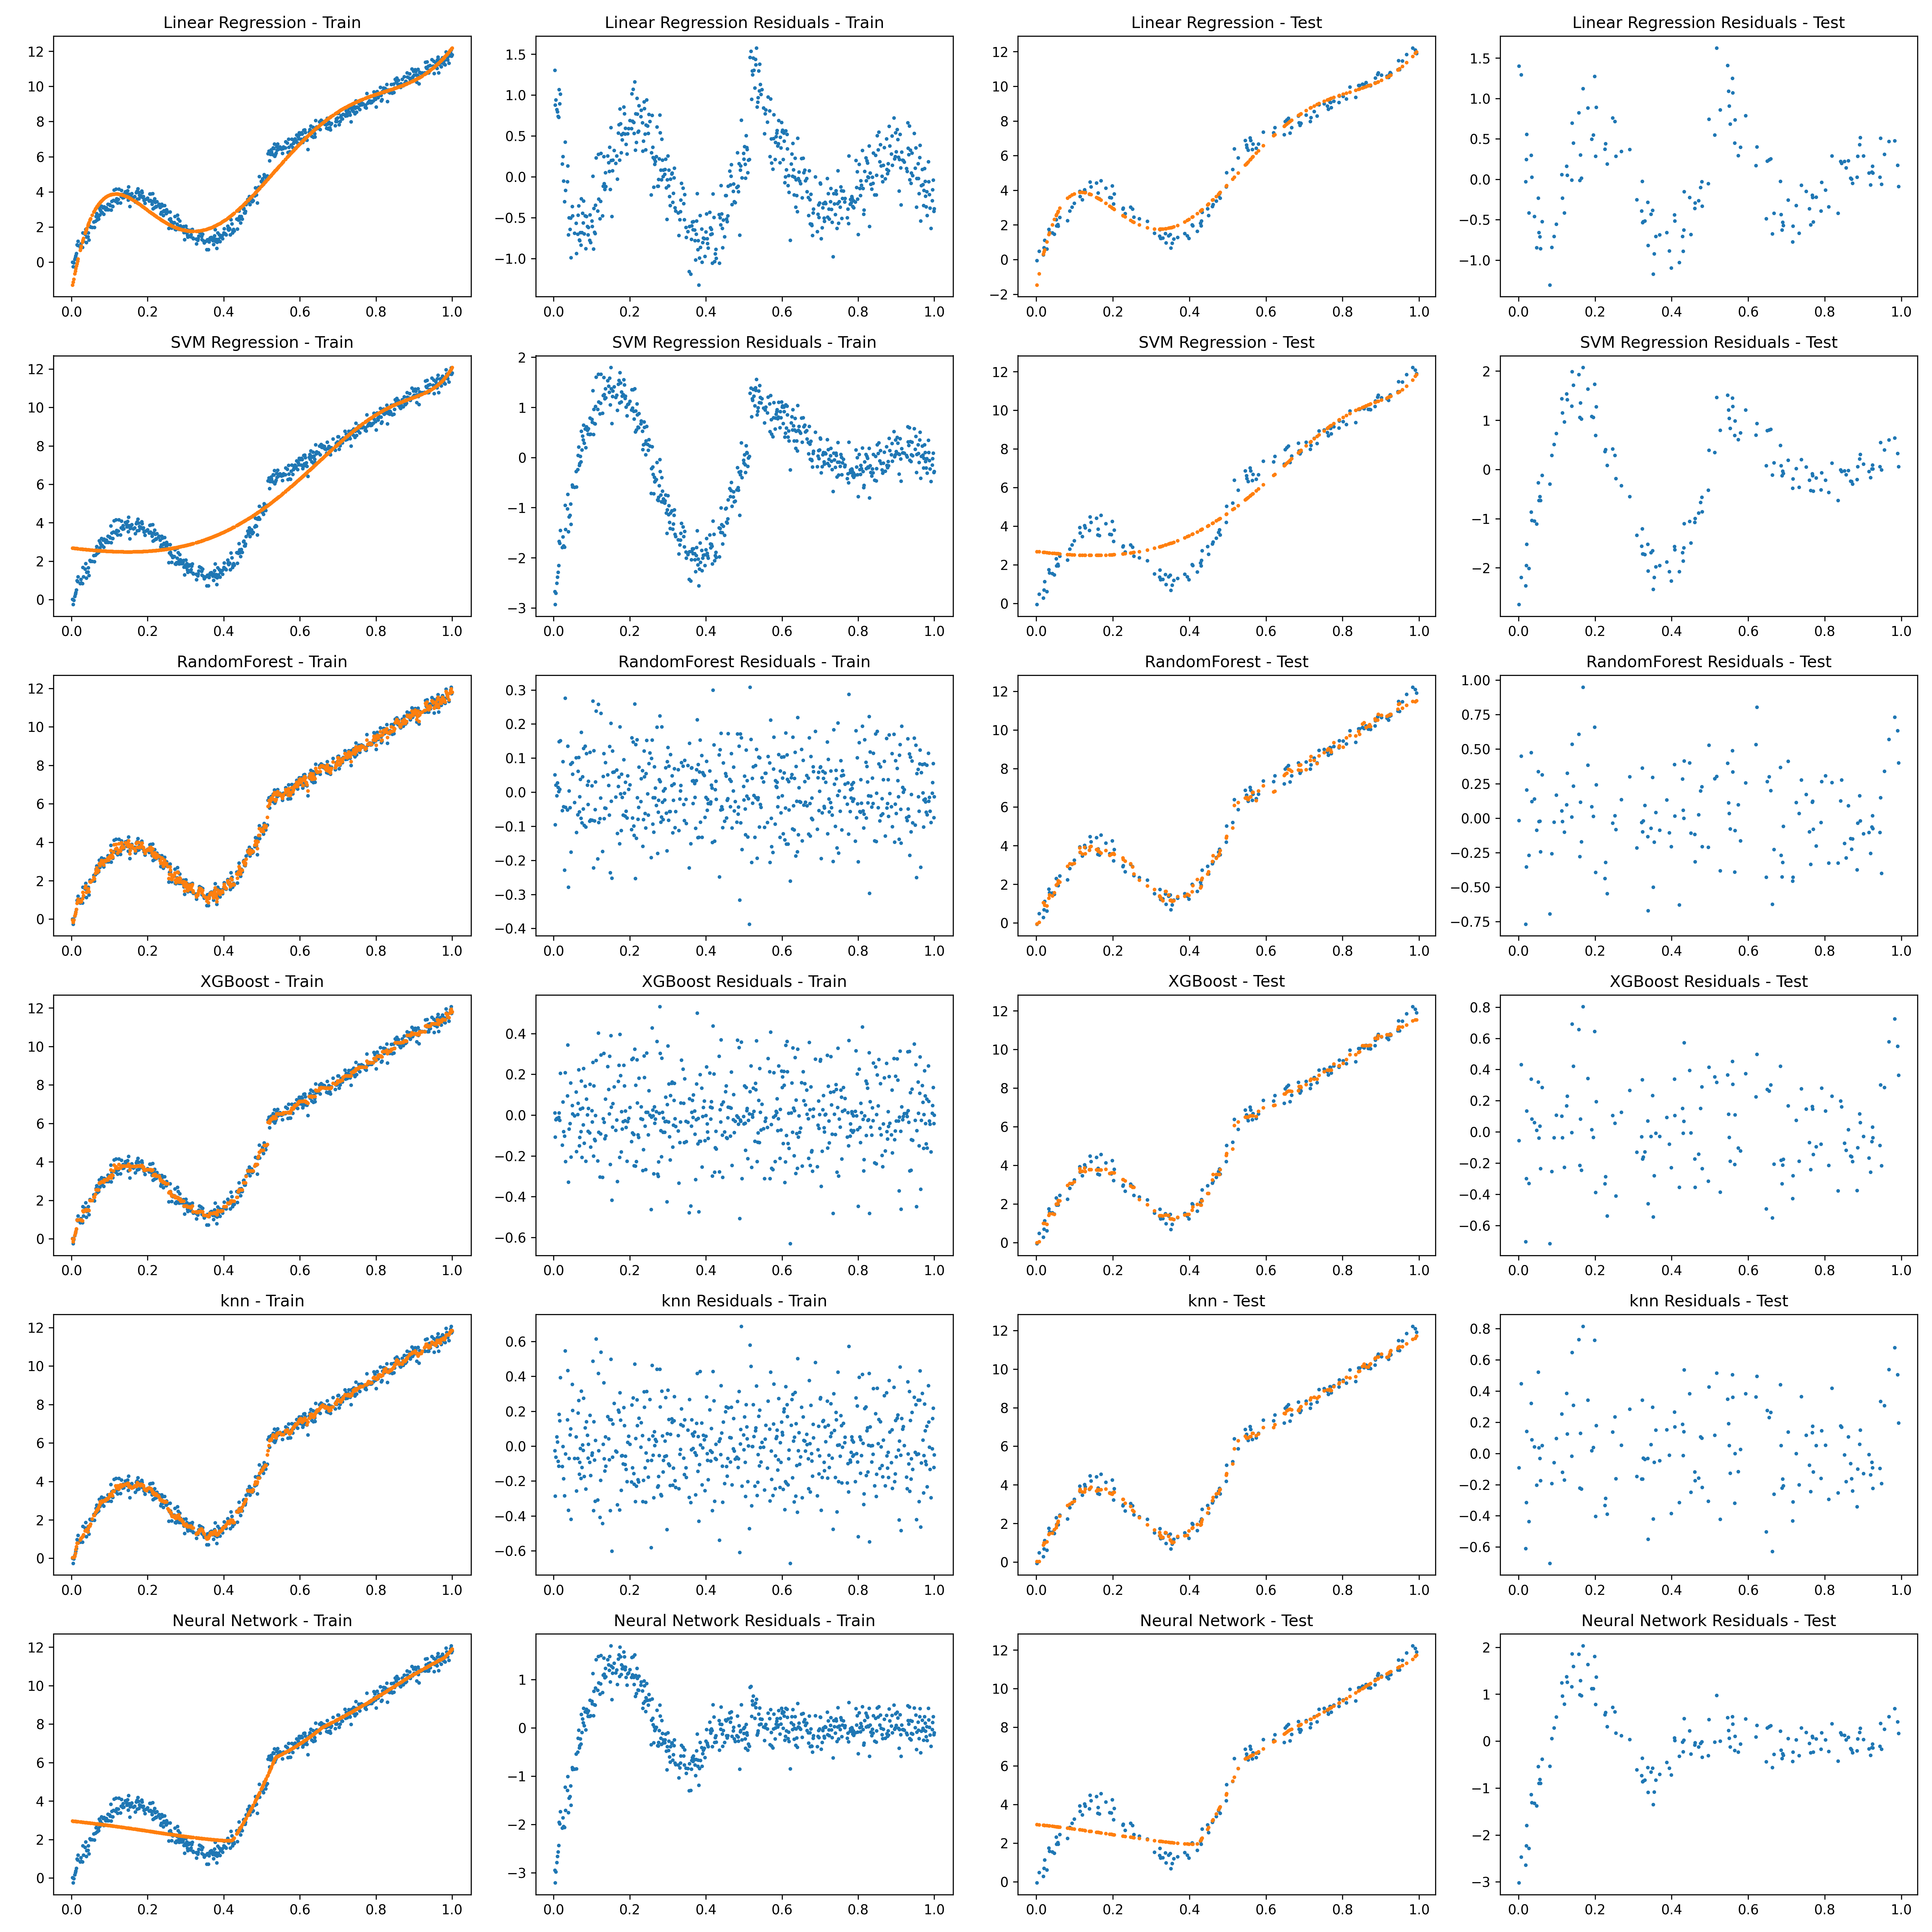
\includegraphics[width=\linewidth]{./Images/E3-MLR3-6.png}
	\caption{Various Regression Models with degree = 6}
\end{figure}

\begin{figure}[H]
	\centering
	\includegraphics[width=1\linewidth]{./Images/E3-MLR3-10.png}
	\caption{Various Regression Models with degree = 10}
\end{figure}

\clearpage

\begin{custombox2}[label={box:Q3a}]{Question (a)}
	Review the \verb|augmented_data.csv| file generated in each case and document your observations.
\end{custombox2}

\clearpage